\title{\textbf{\Huge Book-taste clustering in goodreads communities}}

\author{{\Large Akanksha Tiwari (A0123476E)} \\
    {\Large Antoine Francois Pascal Creux (A0123427M)}\\
    {\Large Ashish Dandekar (A0123873A)} \\\\
    National University of Singapore,\\
    Singapore
}
\date{\today}

\documentclass[11pt]{article}
\usepackage[margin=1in]{geometry}
\usepackage[english]{babel}
% \usepackage{listingstyle}
\usepackage{graphicx}
\usepackage{caption}
\usepackage{subcaption}
% \usepackage{coz}
\usepackage{url}
\usepackage{array}
\usepackage{multirow}
\usepackage{soul}
\usepackage{amssymb}
\usepackage{hyperref}
% \usepackage[autolanguage]{numprint}



\begin{document}
\maketitle

\section{Detailed Problem Description}
Goodreads is a website launched in early 2007, which lets ``people find and share the books they like and improve the process of reading and learning throughout the world.'' It is the world's largest site for readers and book recommendations with a user base of about 30 million members along with 34 million reviews from 900 million books as recorded in 2015 \cite{goodreads:aboutus}.\\\\
Goodreads provides a multitude of features to its users. It goes beyond the traditional rating and reviewing of books by allowing users to make friends and join and form reading groups based on their literary tastes.
Users can not only see what their friends have read, but they can also meet new people with similar reading interests. They can make recommendations to friends, follow authors, track the books they are currently reading, have read and want to read. In addition, goodreads provides personalized recommendations to book readers by analyzing the user data.\\\\
Our project aims  to detect and study goodreads communities based on the book ratings given by users. Through this analysis we seek to understand whether the communities detected based on similar book tastes are alike to the friends communities formed by users themselves on goodreads and the extent to which these user communities on goodreads exhibit homophily.

\subsection{Assumptions}


% The users who have not provided any ratings for the books that they have read are considered as invalid users and we have eliminated them from our data set. This is because just having read the book does not indicate that the user has liked the book. We also need the rating he has given to the book to know whether he/she likes(high rating) or dislikes (low rating) the book he has read.\\\\

However, as of now we have considered users who have given rating for at least a single book as valid users. The data set right now stores a 0 rating if a user has read the book but has not provided a rating for it. We are still working on how to resolve this. One possible way could be to remove this edge between the user and the book. This again could be debatable as by removing this edge we are losing the information that there is a relation between this user and book.\\\\
The users with private profiles whose data we could not scrape because their reading information is just visible to their friends are also considered as invalid users. So, we have not included them in our data set.\\\\
We are assuming that the data we get from scraping is unbiased. That is, we assume that the group ({\it Goodreads Authors/Users}) whose members, members' friends and their books read that we have scraped is representative of readers from various genres. Indeed, this group is very large and popular and is used to share book experiences across different genres.

\section{Related work}

% http://onlinelibrary.wiley.com/doi/10.1002/wics.1319/pdf
% Advanced Review Community detection in large-scale networks: a survey and empirical evaluation
Finally, we also studied different community detection algorithms. Tens of them, if not hundreds exist in the social network analysis field. We do not aim at creating, customizing or optimizing our own algorithm. Given the size of our basic user graph ($86000$), we opt to look for community detection algorithms in large-scale networks.
Many algorithms have arisen in the last few years, as specified in \cite{survey}.
% More about commubnity detection
% Overlapping
% Group based, member based
% What algos do we choose and why?
% Maybe wait for results

% Ashish - Akansha ?



\section{Description of data collection and pre-processing}
\label{sec:data_acquisition}

\subsection{Data collection}
\label{sec:data_colection}

% Goodread provides well documented and publicly accessible API to query various features supported by the website. All we need is a developer key, which one gets after signing up on goodreads, and an OAuth access to use numerous APIs. The data of the users on a website, being the concern of privacy, is not readily available by means of goodread APIs. Aside from this a goodread user has liberty to keep his/her profile private making it accessible only to the friends on goodreads. Given the large user-base of goodreads, we hope to get sizable dataset to run our analysis.\\\\
% Although the data scraping is laborious and time consuming, its is vital in our study. For a fair study, the data must be unbiased. The method which we use to gather the data may add some bias to it. So selection of scraping method is critical to data acquisition. There are two ways one can collect the data:

Even if Goodreads provides well documented and publicly accessible APIs, it is difficult to extract a sample of Goodreads data. For instance, Goodreads do not provide an effortless and unlimited access to reviews of a book.
Anyhow, we have decided to use \emph{reading groups} to obtain a user sampling, representative of Goodreads data.
Indeed, Goodreads hosts various reading groups catered to various genres and reading interests. User can become member of such groups or can initiate a group. In a group reading activities are supported wherein members can schedule the book readings so that they can share their opinions and conduct a healthy conversation. {\it Goodreads Authors/Readers} is one of the major groups on goodreads.  According to goodreads, this group is dedicated to connecting readers with goodreads authors. The description is vague and does not target a specific group of readers.
% It is divided by genres, and includes folders for writing resources, book websites, videos/trailers, and blogs. \\

This is why the members of this group serve as a base user set.
To collect more users, and thus create a substantial dataset, we study the {\it 1-neighborhood} of this set of users, i.e.\ their friends.\\
At the end, we have scraped the ratings of more than 80000 members including more than 1.5 million reviews.

\subsection{Statistics}

An overview of the goodreads data we have scraped is vital as it helps us understand and grasp insight of the data we are munging.
As it is explained in section~\ref{sec:data_colection}, we have extracted our data in two steps:
\begin{itemize}
\item Members of the Goodreads Authors/Users
\item Friends of the Goodreads Authors/Users members
\end{itemize}

\begin{table}[ht]
\begin{center}
\begin{tabular}{lcccc}
\hline
                           &  Goodreads Authors/Users    &   Friends                &   All        \\ \hline
\#Ratings                  &  567461                     &   13832047               &   14399503  \\ \hline
\#Users                    &  17583                      &   95503                  &   113086     \\ \hline
\#Public Profiles          &  7816                       &   78723                  &   86538     \\ \hline
\#Private Profiles         &  2564                       &   5314                   &   7878      \\ \hline
\#Profiles w/o any reviews &  7203                       &   11559                  &   18762      \\ \hline
\#Books rated              &  171653                     &   11559                  &   1714613      \\ \hline
\end{tabular}
\end{center}
\caption{Goodreads Authors/Users Statistics} \label{table:crawl_stat}
\end{table}

% Problem with private profiles. Need data from 100 to 350 for 1st degree connection

As we can see, by getting only the first degree connection of 20000 thousand members, we have almost 15 million reviews, 1714613 books and 86000 reviews posters to analyze.
We first analyze the distribution of the data we have.
Users have read an average of $166$ books, while a book has been read by around $8$ people. 

As expected, half users have read less than 50 books according to Figure~\ref{fig:readers_book_read}. Besides, just like other such as music or movies, users read the same book. Indeed, according to Figure~\ref{fig:books_books_read}, half of the books has been read by only one person. Just $10$\% of books have been read by more than $10$ readers. This highlights the difference of books.

About the ratings, users have given an average rating of $3.52$ while books have an average of $3.23$. This difference, even tiny, strenghens the correlation that a well rated book is more likely to be read.

% print c.user_average_book()
% print c.book_average_user()
% print c.user_average_rating()
% print c.book_average_rating()

% 166.39514433
% 8.38730595677
% 3.524460734
% 3.22690806765

\begin{figure}[ht]
        \centering
        \begin{subfigure}[b]{0.5\textwidth}
                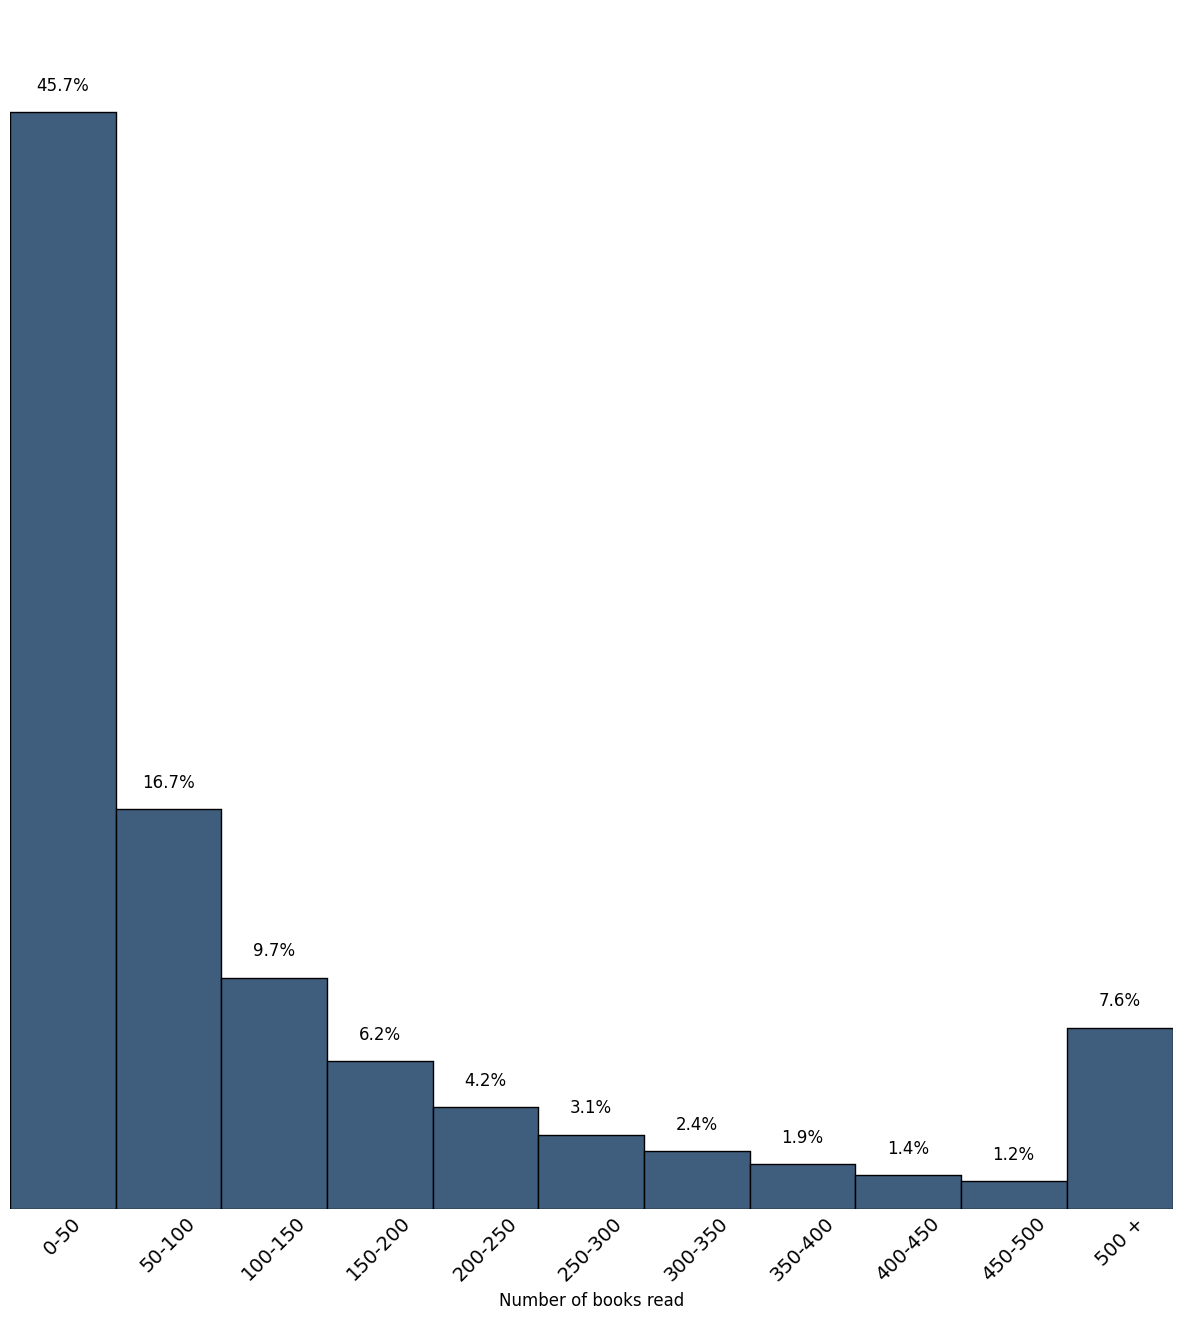
\includegraphics[width=\textwidth]{images/users}
                \caption{Distribution of readers per books read}
                \label{fig:readers_book_read}
        \end{subfigure}%
        ~ %add desired spacing between images, e. g. ~, \quad, \qquad, \hfill etc.
          %(or a blank line to force the subfigure onto a new line)
        \begin{subfigure}[b]{0.5\textwidth}
                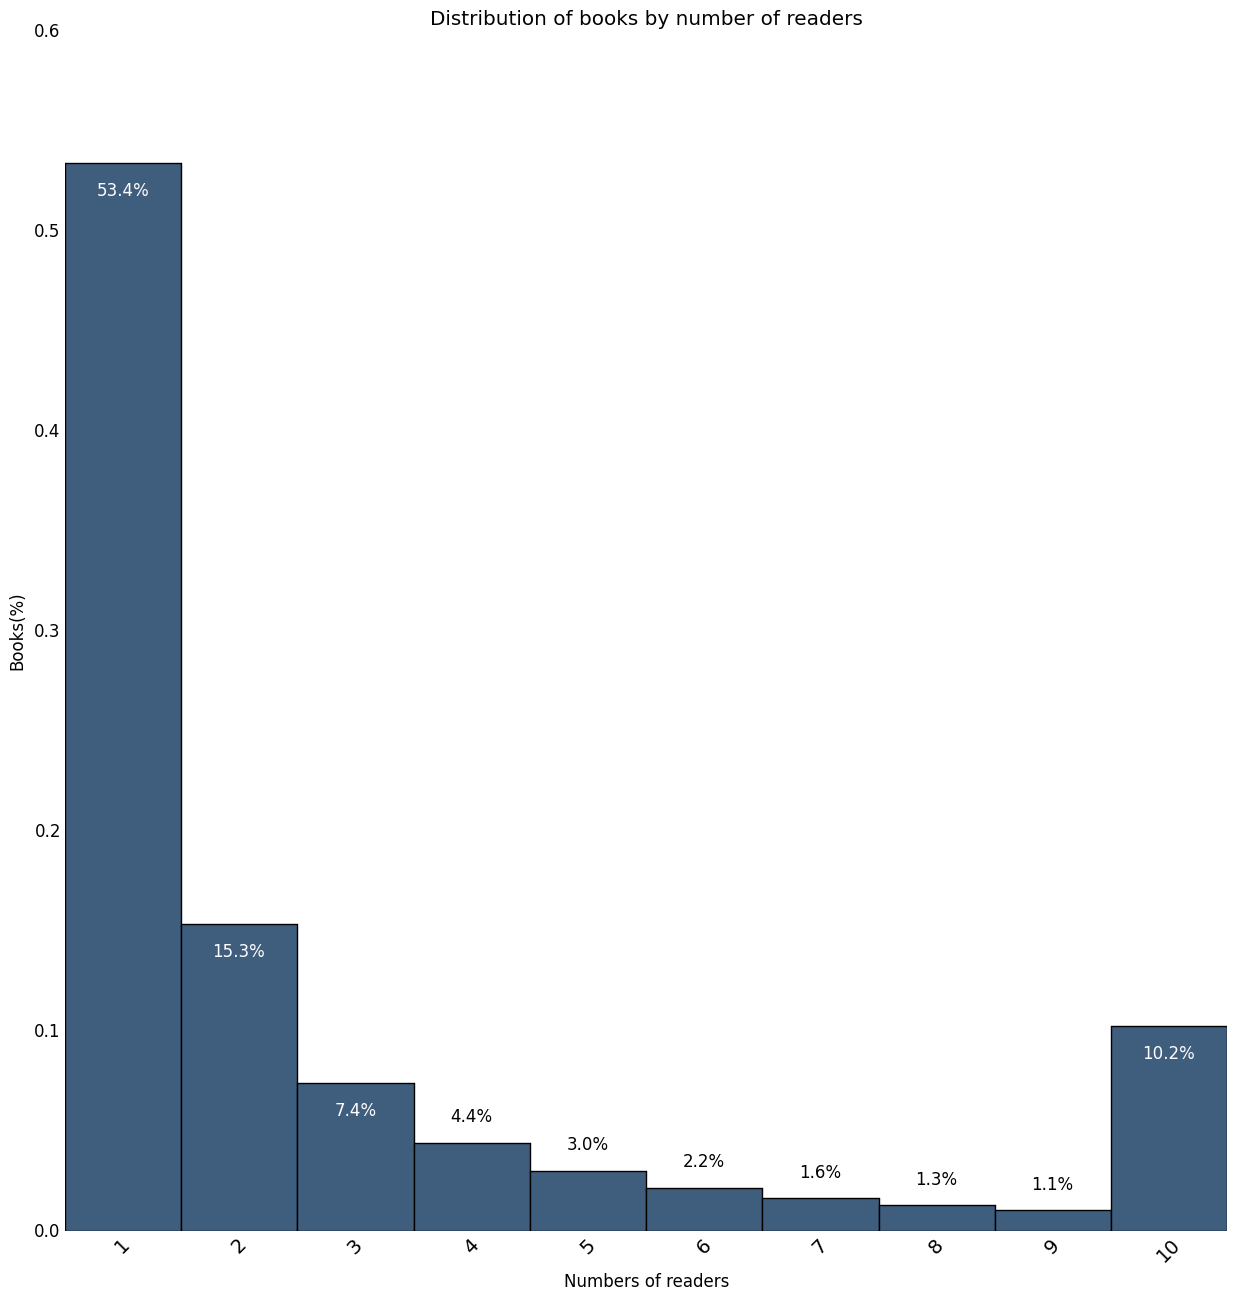
\includegraphics[width=\textwidth]{images/books}
                \caption{Distribution of books per readers}
                \label{fig:books_books_read}
        \end{subfigure}
        \caption{Distribution of books and readers}
\end{figure}

% Books read: 1714613

% !!!!!!always fix bucket size of the column depending on the data!!!!

% User to book
% ------------

% column chart 
% average How many books a user has read - - I want total average



\begin{figure}
        \centering
        \begin{subfigure}[b]{0.5\textwidth}
                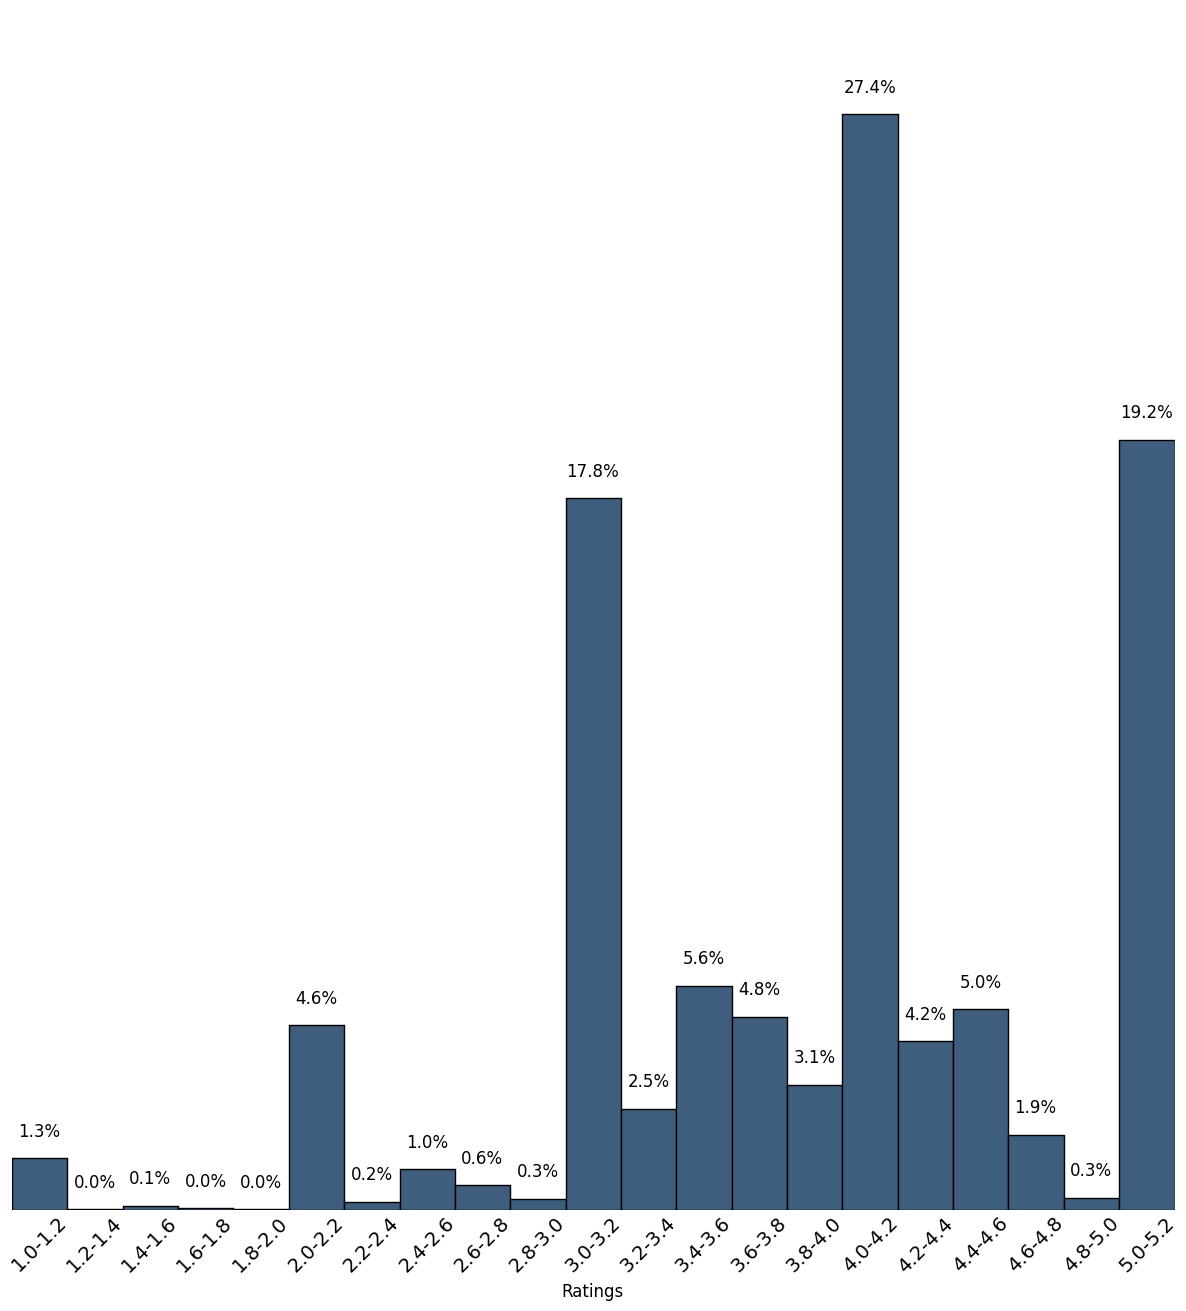
\includegraphics[width=\textwidth]{images/books_ratings}
                \caption{Distribution of books}
        \end{subfigure}%
        ~ %add desired spacing between images, e. g. ~, \quad, \qquad, \hfill etc.
          %(or a blank line to force the subfigure onto a new line)
        \begin{subfigure}[b]{0.5\textwidth}
                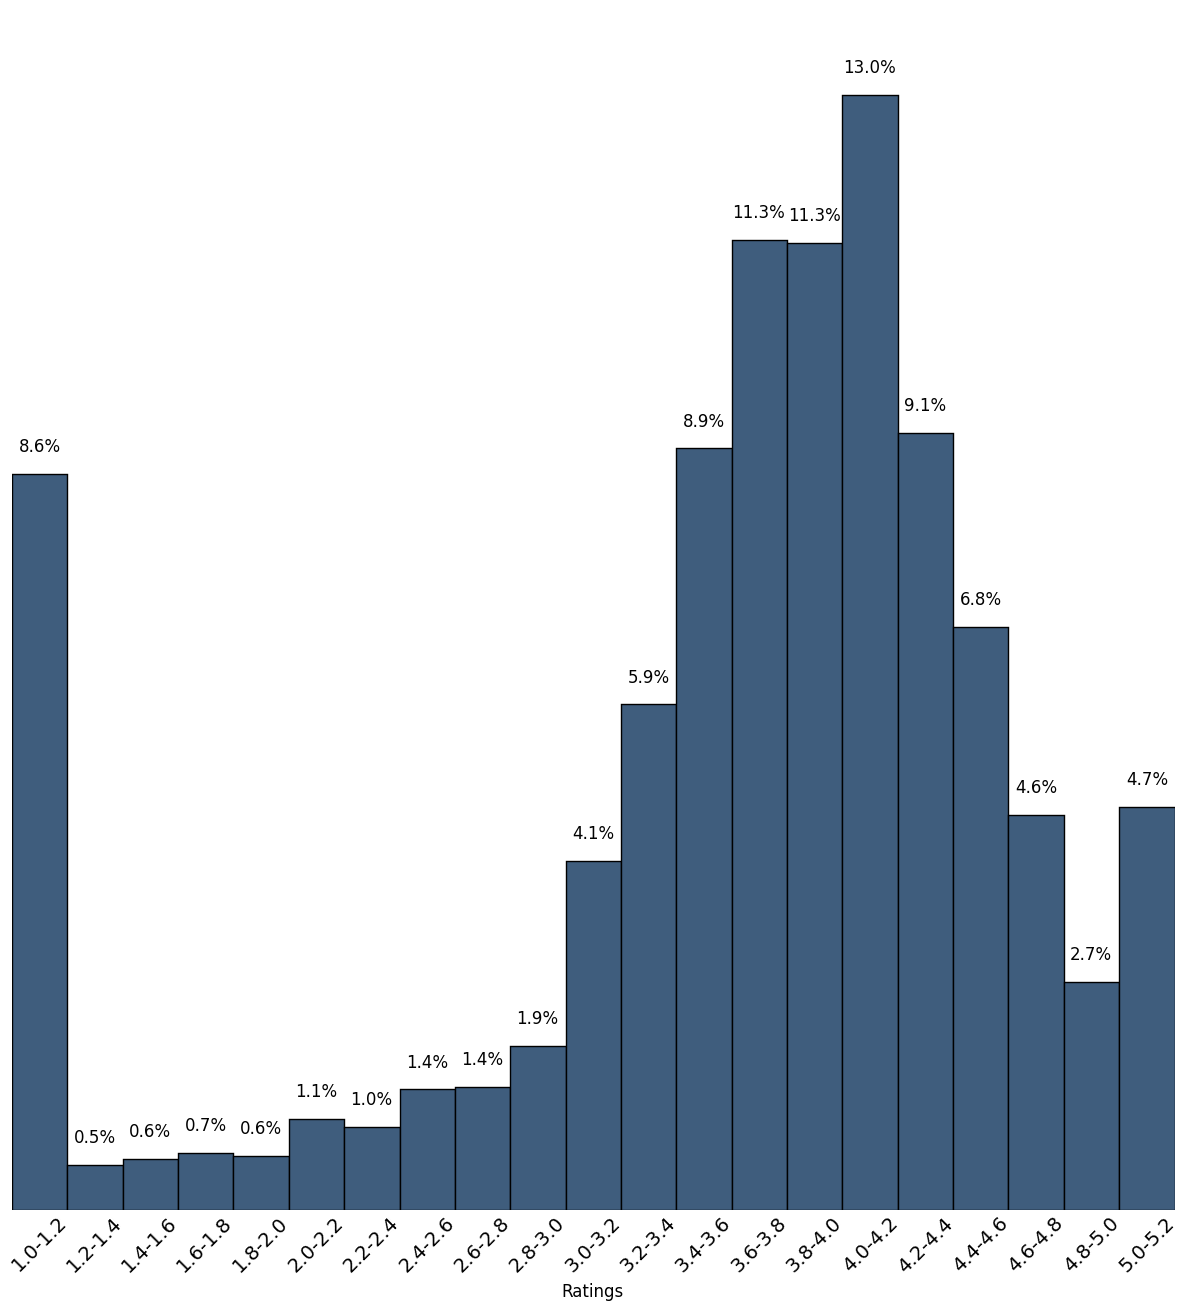
\includegraphics[width=\textwidth]{images/user_ratings}
                \caption{Distribution of readers}
        \end{subfigure}

        \begin{subfigure}[b]{0.5\textwidth}
                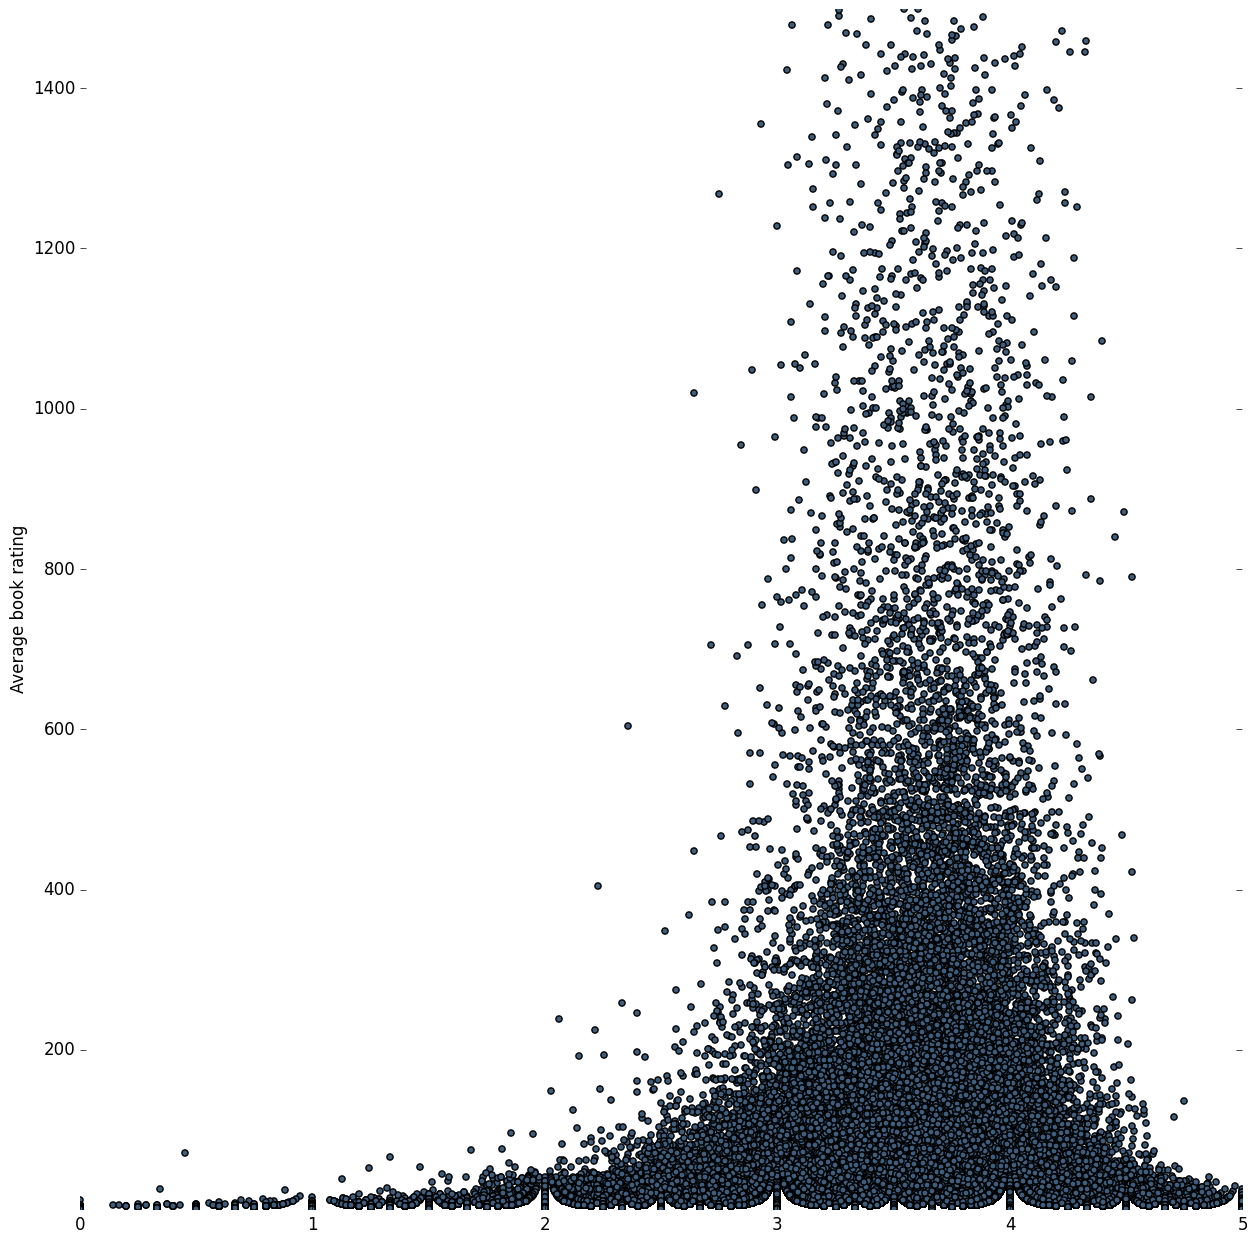
\includegraphics[width=\textwidth]{images/book_scatter_1500}
                \caption{Books per rating}
        \end{subfigure}%
        ~ %add desired spacing between images, e. g. ~, \quad, \qquad, \hfill etc.
      %(or a blank line to force the subfigure onto a new line)
        \begin{subfigure}[b]{0.5\textwidth}
                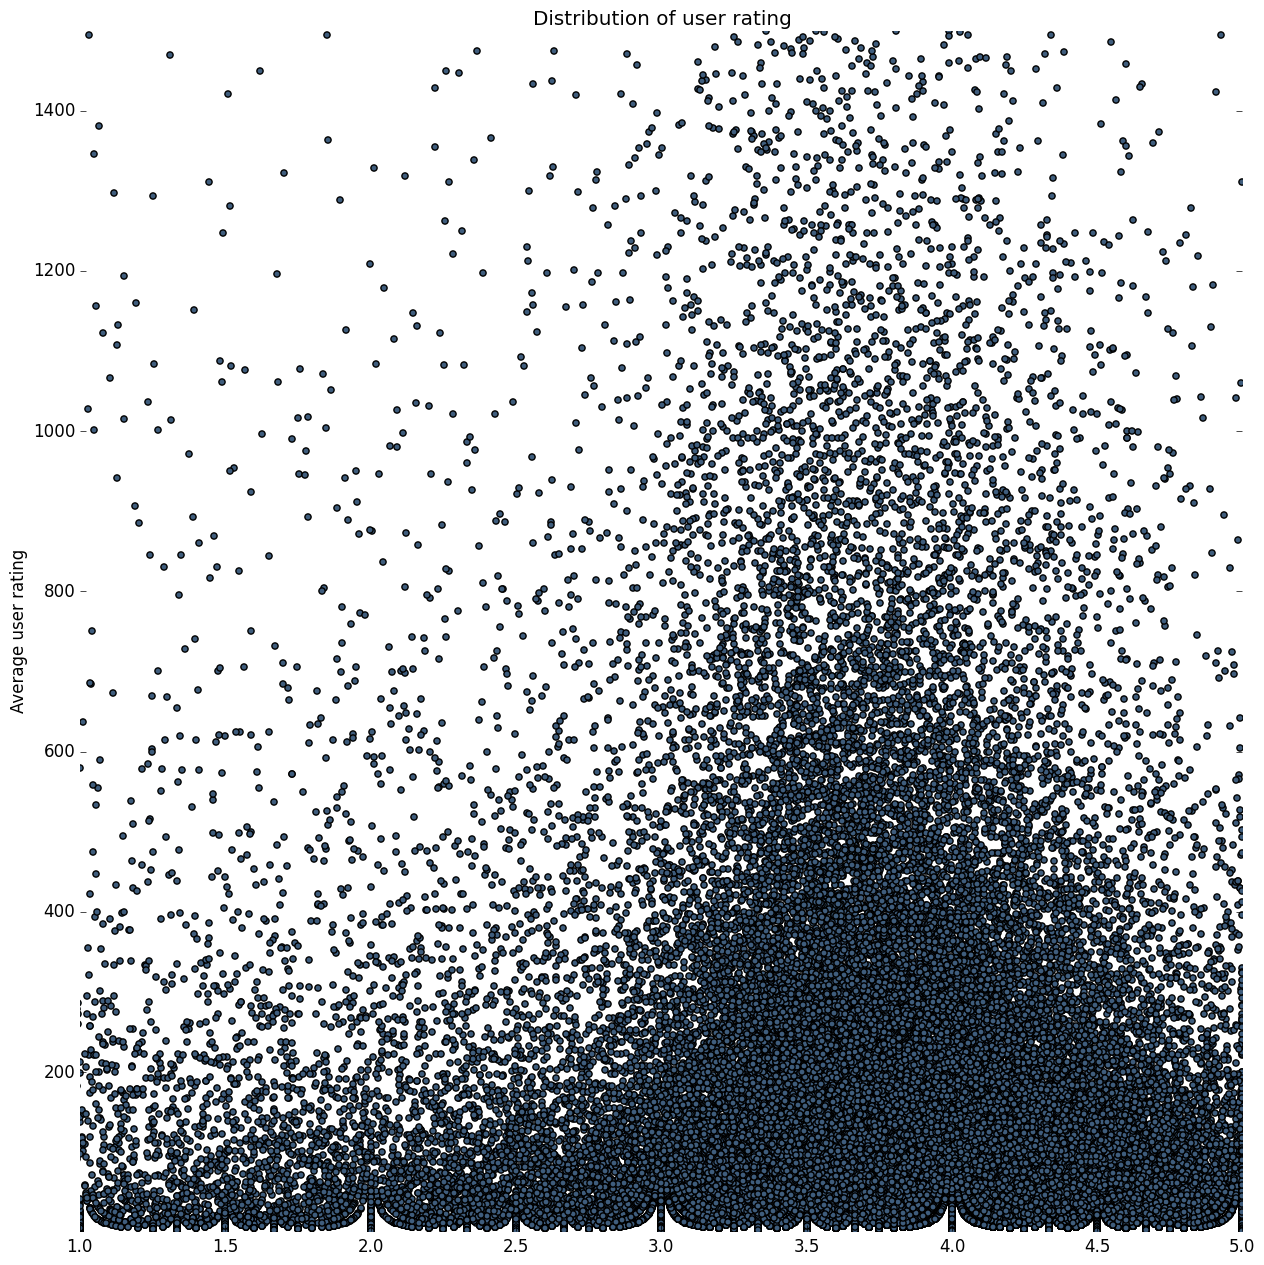
\includegraphics[width=\textwidth]{images/user_scatter_1500}
                \caption{Readers per rating}
        \end{subfigure}
        \caption{Distribution of ratings for readers and books}
        \label{fig:scatters}
\end{figure}

About the distribtion of ratings, both books and readers have a similar distribution as seen in Figure~\ref{fig:scatters}.

% \begin{figure}
%         \centering
%         \begin{subfigure}[b]{0.4\textwidth}
%                 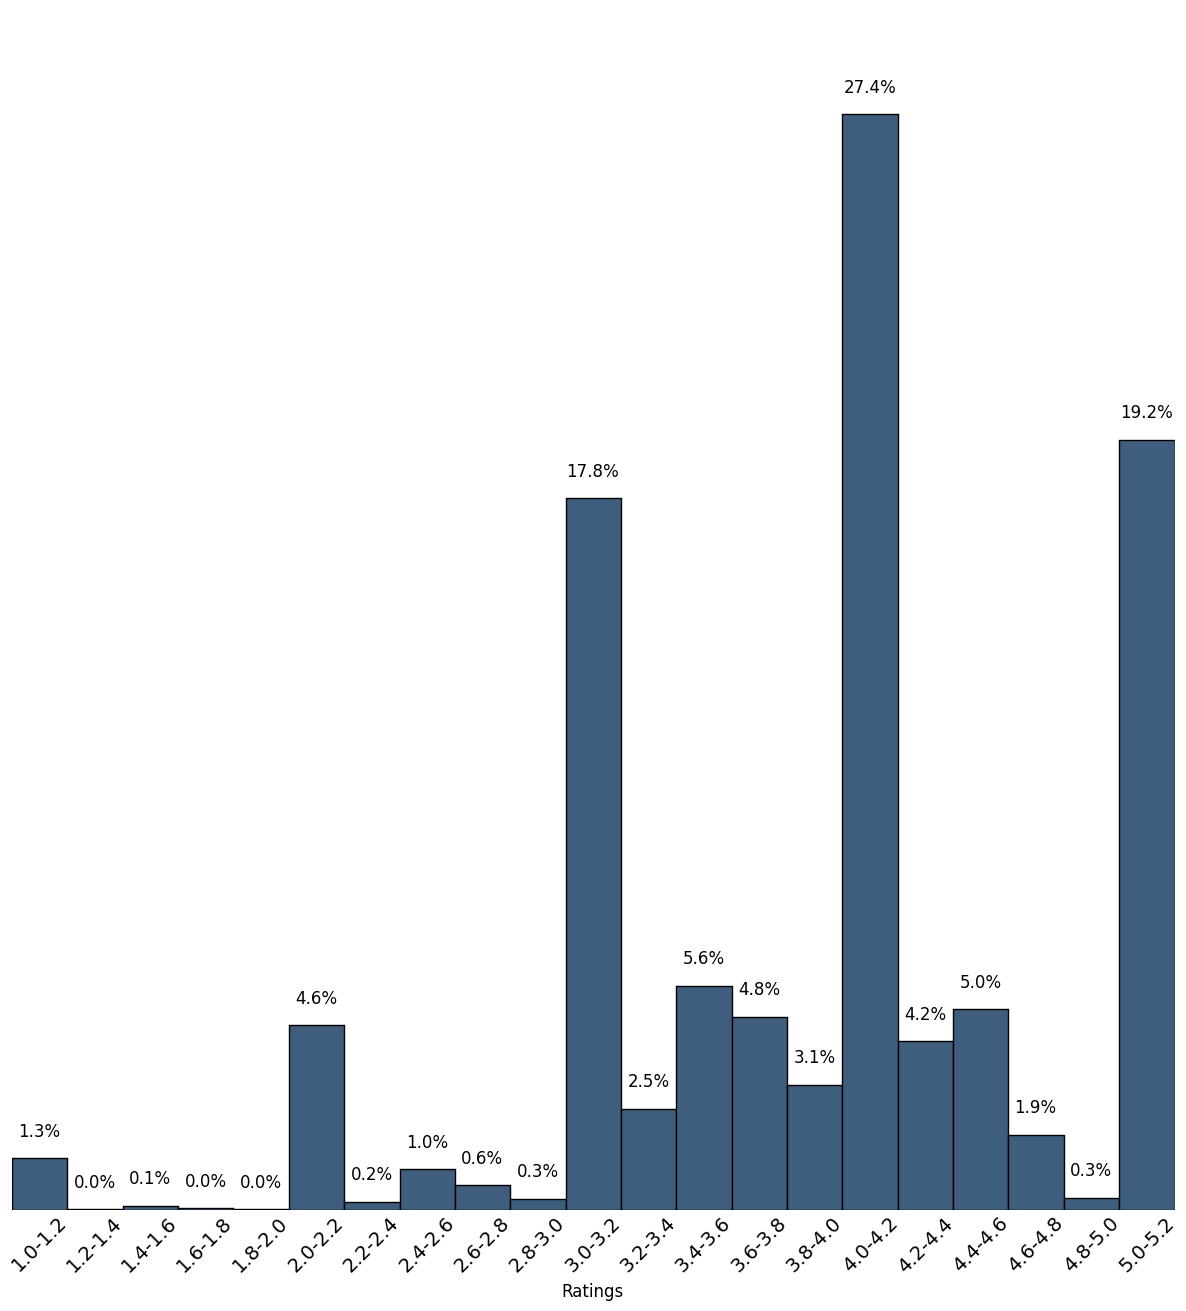
\includegraphics[width=\textwidth]{images/books_ratings}
%                 \caption{Distribution of books}
%         \end{subfigure}%
%         ~ %add desired spacing between images, e. g. ~, \quad, \qquad, \hfill etc.
%           %(or a blank line to force the subfigure onto a new line)
%         \begin{subfigure}[b]{0.4\textwidth}
%                 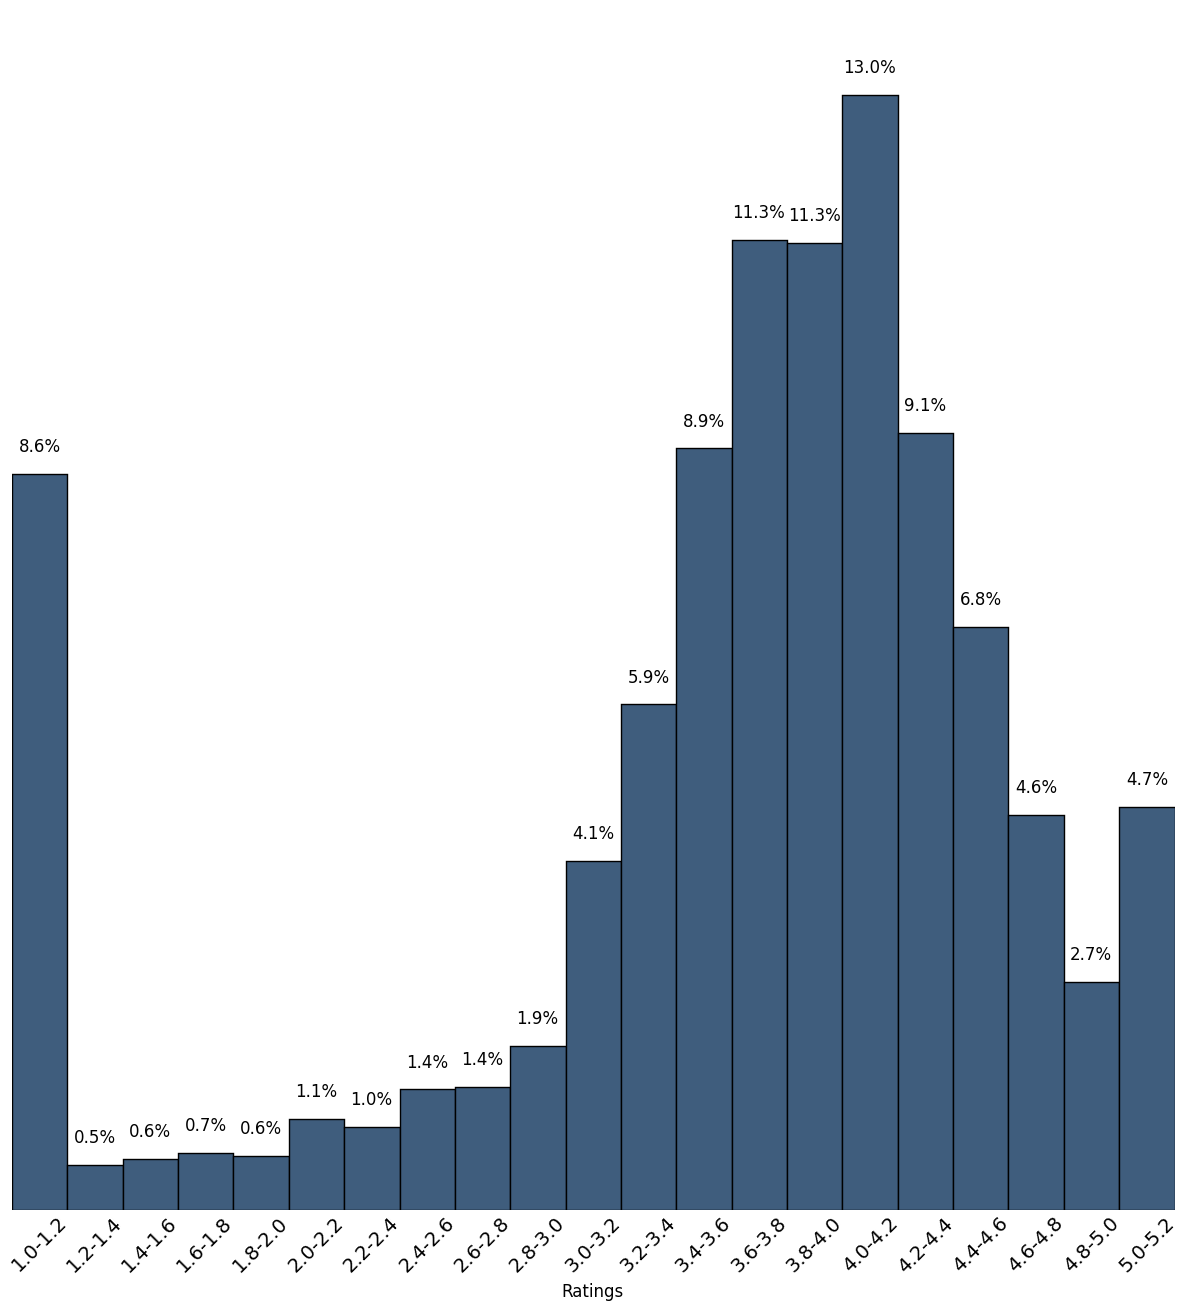
\includegraphics[width=\textwidth]{images/user_ratings}
%                 \caption{Distribution of readers}
%         \end{subfigure}

%         \begin{subfigure}[b]{0.4\textwidth}
%                 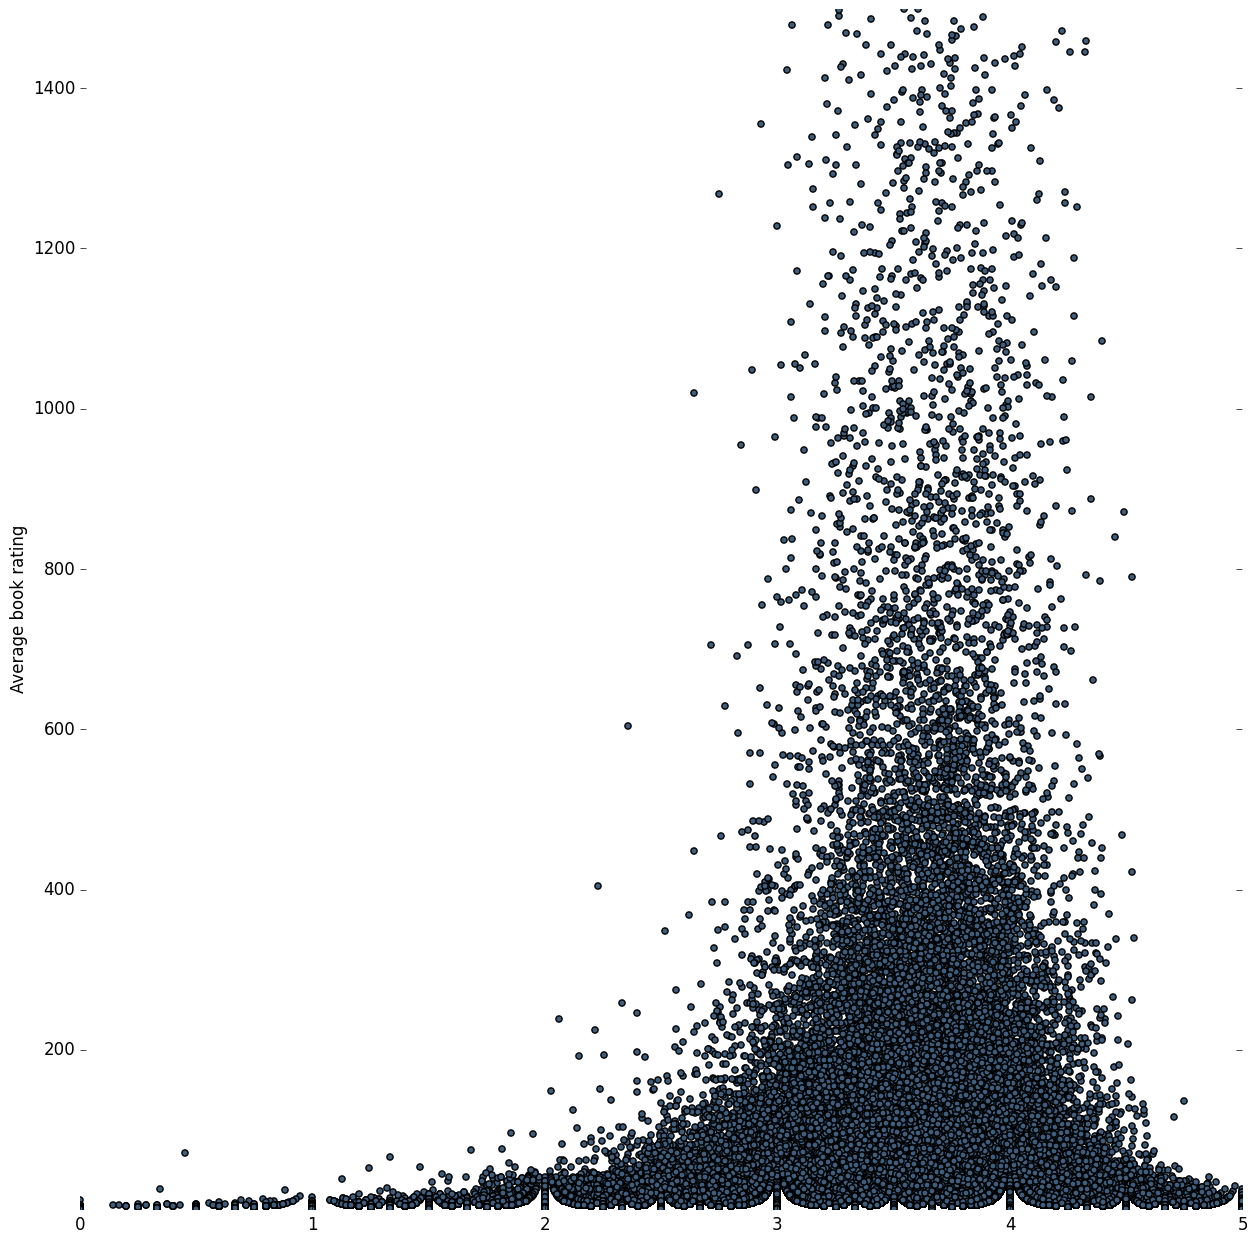
\includegraphics[width=\textwidth]{images/book_scatter_1500}
%                 \caption{Books per rating}
%         \end{subfigure}%
%         ~ %add desired spacing between images, e. g. ~, \quad, \qquad, \hfill etc.
%           %(or a blank line to force the subfigure onto a new line)
%         \begin{subfigure}[b]{0.4\textwidth}
%                 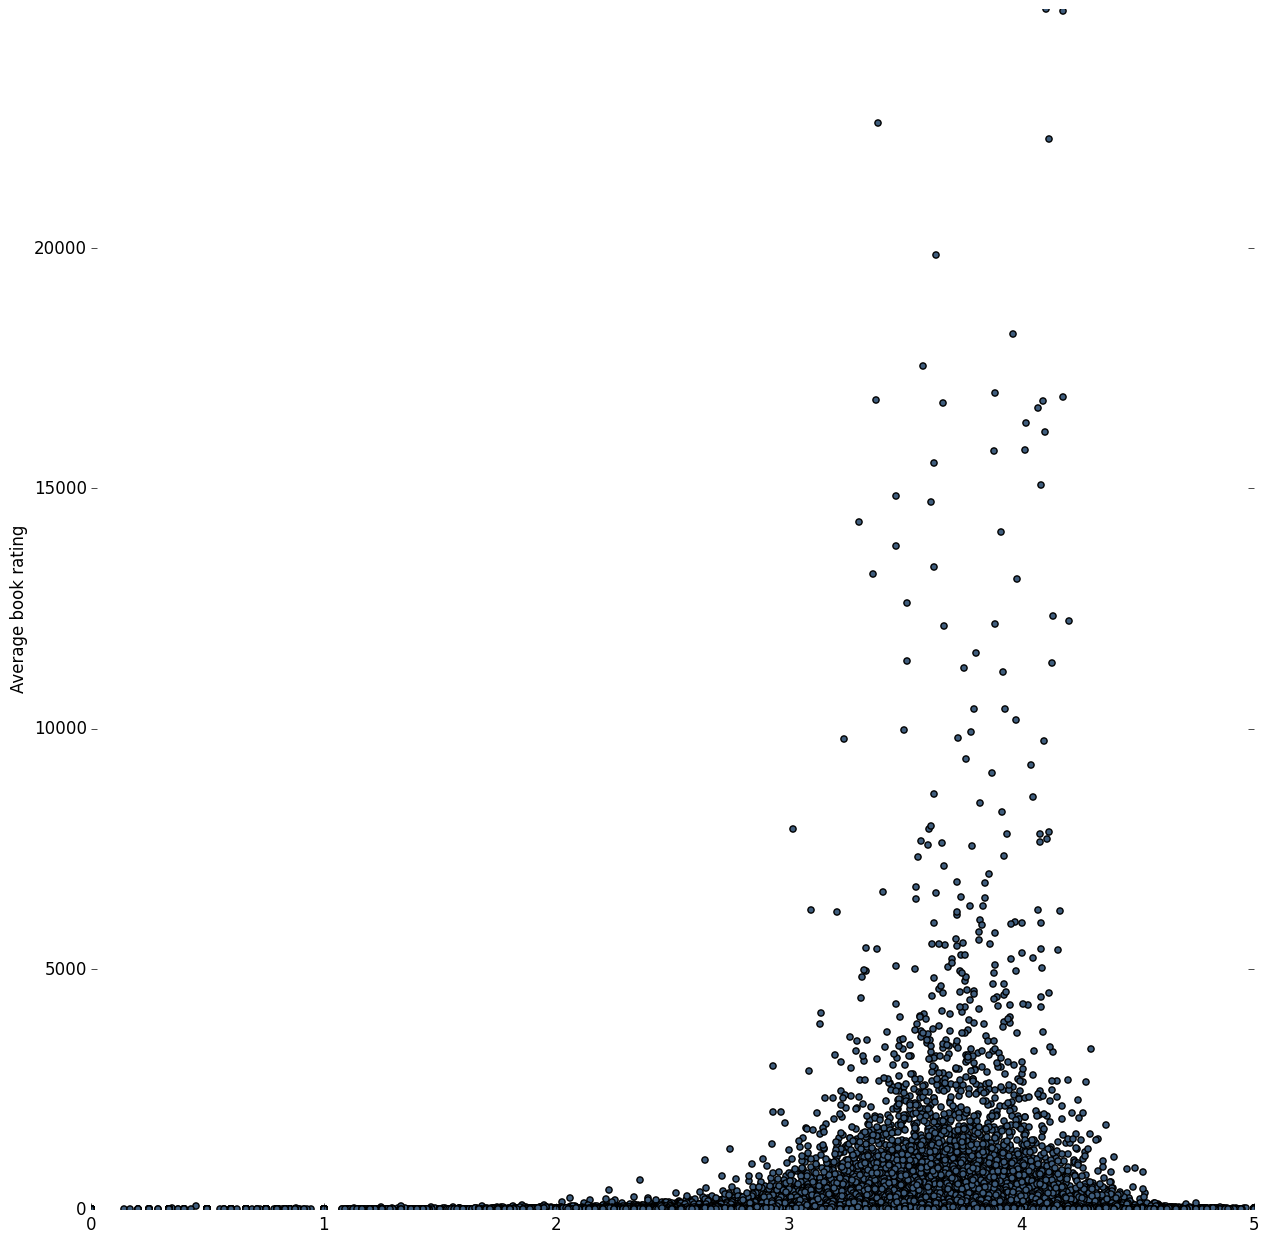
\includegraphics[width=\textwidth]{images/book_scatter}
%                 \caption{Books per rating}
%         \end{subfigure}

%         \begin{subfigure}[b]{0.4\textwidth}
%                 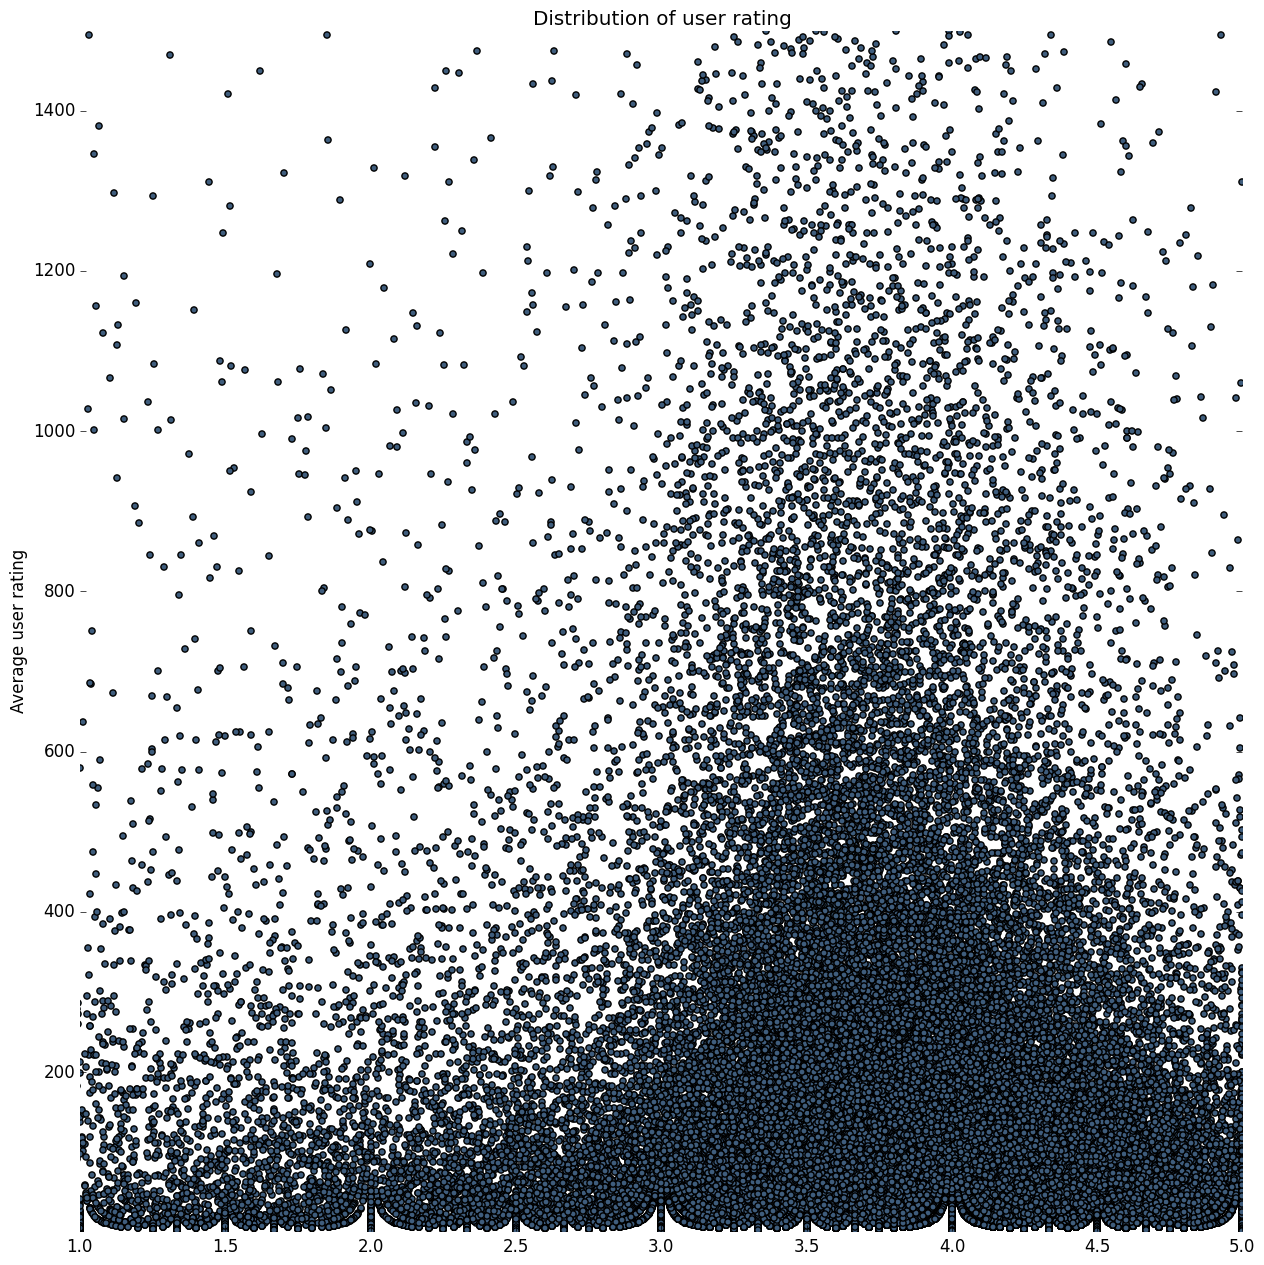
\includegraphics[width=\textwidth]{images/user_scatter_1500}
%                 \caption{Readers per rating}
%         \end{subfigure}%
%         ~ %add desired spacing between images, e. g. ~, \quad, \qquad, \hfill etc.
%           %(or a blank line to force the subfigure onto a new line)
%         \begin{subfigure}[b]{0.4\textwidth}
%                 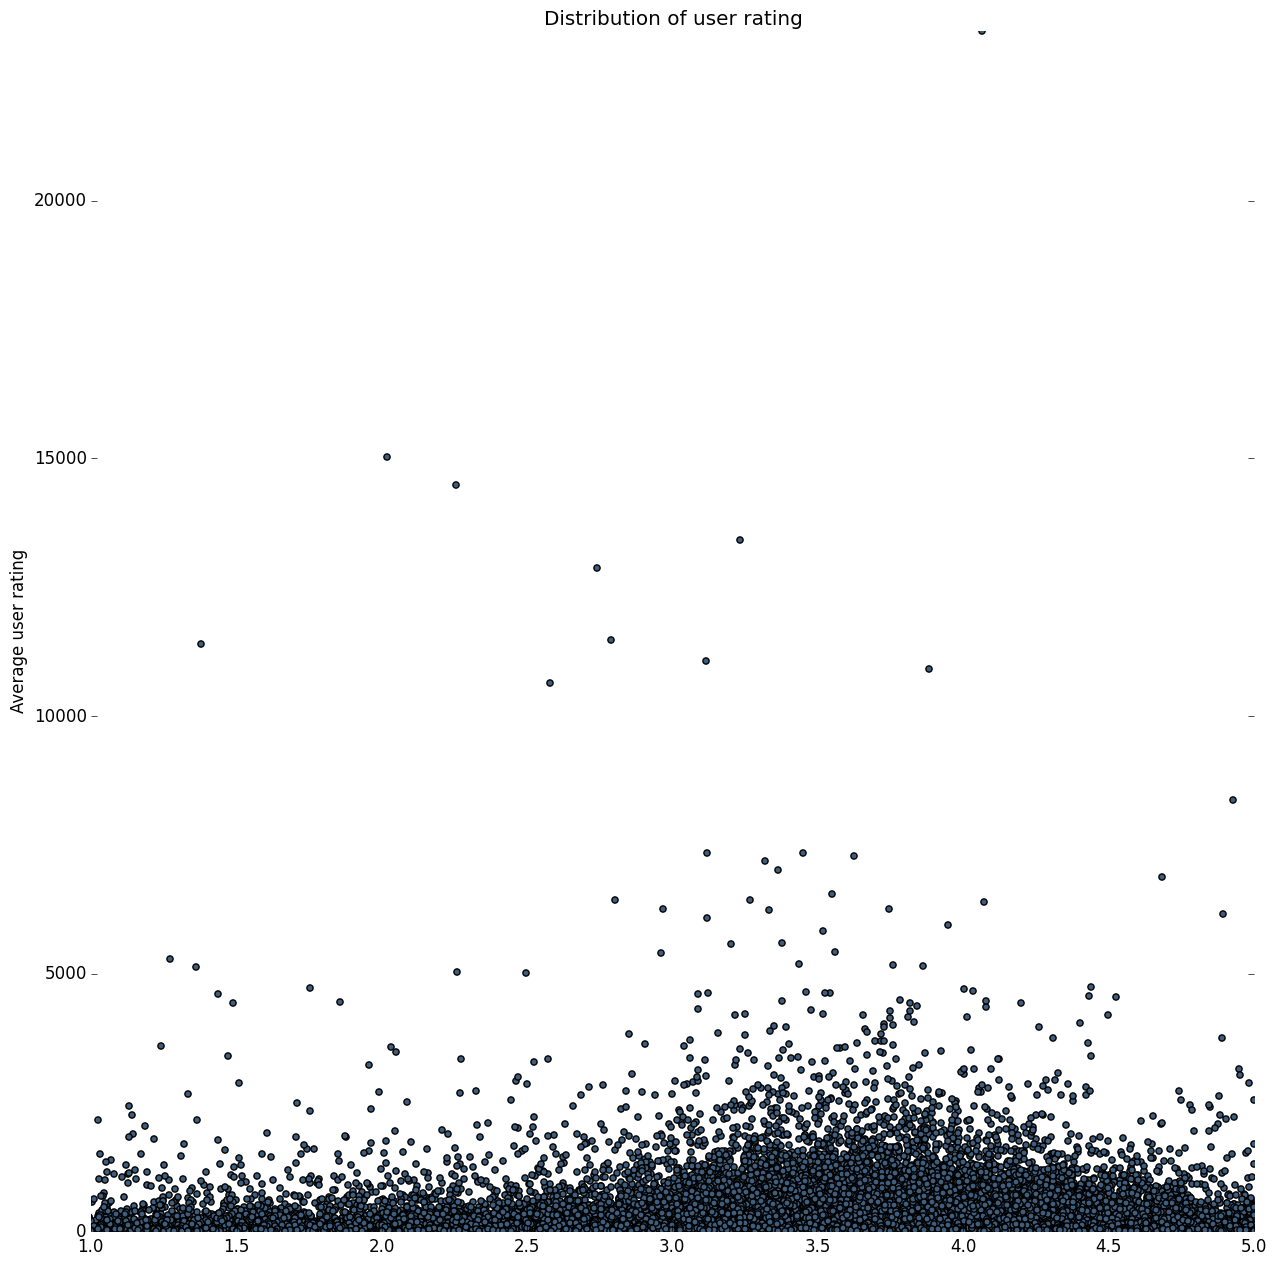
\includegraphics[width=\textwidth]{images/user_scatter}
%                 \caption{Readers per rating}
%         \end{subfigure}
% \end{figure}


% book_scatter_1500.png
% book_scatter.png
% books.png
% books_ratings.png
% user_ratings.png
% user_scatter_1500.png
% user_scatter.png
% users.png

% print c.user_average_book()
% print c.book_average_user()
% print c.user_average_rating()
% print c.book_average_rating()

% 166.39514433
% 8.38730595677
% 3.524460734
% 3.22690806765


% distribution - column chart - 10 buckets (0-10, 11-20, 21-30... 80+) -> fix bukcet size depending on the data

% column chart 
% Average rating a user has given - - I want total average
% distribution of a user -average rating - column chart - 10 buckets (0.1-0.5, 0.6-1... 4.5-5)

% Graph:
% x -> Nb of books read by a user
% y -> Average rating given by a user
% 1 point = 1 user


% Book to user
% ------------

% column chart 
% average readers for 1 book - I want total average
% distribution - - 8 buckets (0-1000, 1001-2000, ...8000_+) -> fix bucket size depending on the data

% column chart 
% Average rating for a book - I want total average
% distribution of a book-average rating - column chart - 8 buckets (0.1-0.5, 0.6-1... 4.5-5)

% Graph:
% x -> Nb of ratings
% y -> Average rating given to the book
% 1  point = 1 book


\section{Description of the model, algorithm, and/or core of project}

The objective of the project is to determine that the friends graph captures the homopholy based on the book preferences.
Indeed, ...
% Ashish

Our data enable us to compute the weight of an edge between any two users. The most simple and common way to do this is to compute the projection matrix. For instance, it is normal to consider no edge between two users who have not read any common book. Due to performance issue and based on our assumption, we wanted to interpret the edge between two users. We tried different kinds of scoring functions, some of them were supposed to capture better the homophily.
Among those scoring functions, some were more focused on the rating, some on books both users have very liked, or just the number of books they have read in common.

% Detail the scoring functions?

% Community detection Algorithms
% What did we choose and why?






\section{Discussion of key challenges}

Many challenges arose during this study, and we needed to fix each bottleneck simultaneously.

\subsection{Data processing}

During data scraping, we needed to request many times the Goodreads APIs.
We had decided to retrieve the users of a reading group, get all the reviews from each user and retrieve all friends for each user.
Each information retrieval is one request sent to Goodreads APIs.
By storing almost $90000$ users, we made more than 1 million requests. Using multiprocessing, we speed up this part but make data storage more complicated and difficult to read.

\subsection{Matrix projection}

With $90000$ users, $1.7$ million books and $14$ million reviews, we need to project this bipartite graph to a user-user graph.

The user-book matrix, named $R$, of shape $90000 \times 1700000$, is very sparse as its density is around 0.001. But the projection matrix was too dense, as two users who have read the same book might be related in the reader graph.
The projection user-graph is computed as: $U~=~R \dot R^T$.
We tried computing $U$ using \emph{sparse} matrices within the well-known library \emph{Scipy}\cite{scipy}, but we hit a memory overflow on a 64GB machine.
Besides, a $90000 \times 90000$ matrix of short integers requires $32$GB and thus does not fit in a laptop memory.

So we chose two ways to deal with it:
\begin{itemize}
\item Using a sample of users. We can deal with 10000 users and keep meaningful insights of our analysis.
\item Filter the edges created. If two users have read 1000 books each, and they only have rated one book in common, we do not need to create an edge between those both users. Computing a too dense user graph is time-wasting and does not give relevant information.
\end{itemize}

\subsection{Projection}

Using a matrix projection is a very basic way of interpreting relation between two users. To give a meaningful weight between, we compute each edges between two users by hand. A problem raised as we needed to compute the edge weight between every pair of two readers. So, if we want to build a graph with $n$ users, we should compute $\frac{n * (n-1)}{2}$ edges. For 10000 users, we have to compute 50 million edges. Multiprocessing helps us reduce this time by a factor of 10.

\section{Evaluation of your experiments / results / finding}

% based on analysis, _analysis, results.csv, results.ynip





\section{Outline of each team member’s contributions}



% \subsection{Objectives}

% \begin{itemize}
% \item[\checkmark] Gather relevant data (as mentioned in Section \ref{sec:data_acquisition}) from goodreads
% \item[\checkmark] Survey various algorithms for community detection on the graphs generated from the data
% \item Analyze and interpret the results of applying these algorithms on the data 
% \item Analyze the extent to which the user groups on goodreads exhibit homophily
% \item Study the effect of recommendations and users' friend on his/her choice of books (If time permits)
% \end{itemize}

% \subsection{Contribution}
% As of the literature survey done up to now, there has not been a study on the detection of communities of readers with similar reading interests on goodreads dataset.
% This work will aim to identify such communities using algorithms for community detection such as Girvan-Newman algorithm and compare the communities detected with the already formed groups on goodreads and analyze how different or similar they are.
% This would give us insights into whether the friendship and groups formed on goodreads are based on reading interests or there are other factors that come into play. It can be especially useful to authors in identifying the right target audience for their work. \\\\
% In addition, if we get time, we can also look at how the recommendations and friendships in the goodreads' user network affect the choice of books. This information can be used by goodreads themselves to improve their recommendation engine.

% \section{Related Work}
% Our focus is on studying whether the existing groups on goodreads exhibit homophily based on the communities we detect using the user graph generated from the book ratings given by users.Based on the sample we have, the graph is very dense. With less than 8000 user nodes, we have more than 16 million edges. The density is about 50 \%.Community detection is a widely discussed topic in the social networking literature\footnote{Social networks are generally sparse networks. When the networks are dense, the community detection does not seem to be a wise option. The dense networks possess large number of inter-community edges which yield poor partitioning. For dense networks, discrete data analysis techniques are used.}\cite{clauset}. Initially, we decided to use the Girvan-Newman algorithm as it is one of the most popular community detection algorithms\cite{newman}. This algorithm uses the ``edge betweenness'' of an edge as the number of shortest paths between pairs of nodes that run along it. Edges with high betweeness are very likely to be the connection between communities.
% Thus, removing the edges in the decreasing order of betweenness should reveal the associated dendrogram, and thus the communities. However, this computation takes $O(ne)$ running time, and thus is too long for our graph.\\\\
% G-N can be limiting as every node has to be placed in one unique community.
% In order to use this algorithm , since we are dealing with a bipartite graph, we can try to find complete bipartite subgraphs. That is, we can split the users and the books into two distinct sets respectively, such as $users0$ and $books0$, and $users1$ and $books1$ are linked, but no edges connect $users0$ and $books1$, or $users1$ and $books0$. However, based on our graph density which is pretty high, we cannot apply this algorithm: we could end up getting a unique complete clique.However, we could filter the edges.For instance, keeping only the edges with a rating of 5.\\\\

% The Simrank method, where a random walker starts at one node, and is allowed to go through the edges is cannot also be applied to our dense graph.The similarity between each node is too time-consuming. \\\\

% The Louvain\cite{louvain} method for community detection which has come up in the last few years, is a graph partitioning technique that provides an accurate and computationally efficient approach to detect communities in networks consisting of millions of nodes. We will explore this method in the current study.

% \section{Data Acquisition}
% \label{sec:data_acquisition}
% Goodread provides well documented and publicly accessible API to query various features supported by the website. All we need is a developer key, which one gets after signing up on goodreads, and an OAuth access to use numerous APIs. The data of the users on a website, being the concern of privacy, is not readily available by means of goodread APIs. Aside from this a goodread user has liberty to keep his/her profile private making it accessible only to the friends on goodreads. Given the large user-base of goodreads, we hope to get sizable dataset to run our analysis.\\\\
% Although the data scraping is laborious and time consuming, its is vital in our study. For a fair study, the data must be unbiased. The method which we use to gather the data may add some bias to it. So selection of scraping method is critical to data acquisition. There are two ways one can collect the data:
% \begin{description}
% \item[Retrieve User IDs from a group]
% Goodreads hosts various reading groups catered to various genres and reading interests. User can become member of such groups or can initiate a group. In a group reading activities are supported wherein members can schedule the book readings so that they can share their opinions and conduct a healthy conversation. {\it Goodreads Authors/Readers} is one of the major groups on goodreads.  According to goodreads, this group is dedicated to connecting readers with goodreads authors. It is divided by genres, and includes folders for writing resources, book websites, videos/trailers, and blogs. \\
% Goodreads provides an API to get the list of users given the ID of the group. One can get the ID of the group from the URL of the corresponding group on goodreads.
% \item[Retrieve User IDs from reviews of books]
% The list of various books genres is available at \cite{goodreads:genres}. One can select top rated books from the highly reviewed genres. So this collection of ``best-selling'' books forms a base set for the books. So we can get the list of users who have read these books. But goodreads fails to support an API which retrieves reviews for a particular book given its ID. Despite this, a meticulous analysis of \textit{Javascript} calls, the webpage makes to show the reviews of a book to the user, reveals a bacdoor API \textit{book/reviews/}. We can retrieve user related information User ID and the rating by parsing the response to the \textit{Javascript} callback using regular expressions.
% \end{description}
% The list of User IDs thus scraped serve as a base user set. We later collect {\it 1-neighbourhood} of this set of users, namely friends of them and the books read by these friends, to get a substantial dataset.\\
% We have decided to go with the first strategy. By scraping a toy dataset, we observe the data to be unbiased. Plus the data related to the friends assures the sizable amount for the analysis.

% \section{Description of the method}
% Following is the overview of the proposed analysis:
% \begin{itemize}
% 	\item Form a weighted bipartite network of users and books from the data scraped
%     \item Obtain projected users' network from the bipartite network
%     \item Find the communities in the projected users' network
%     \item Synthesize a goodreads friendship network by using the data
%     \item Compare and analyze both the networks to estimate the extent of homophily
% \end{itemize}
% \section{Project Progress}

% To gather a substantial set of users, we collect the friends of the base users. Again, we filter the friends who are already in the group, who have kept their profiles private and the ones who have not reviewed a single book. Following this strategy, we have a consolidated list of 95503 users which will be the user base for out analysis. \\
% The code for scraping is available on \href{https://github.com/acreux/nus-cs5345-project/tree/dev}{Github}. To speed up the scraping process, we have also implemented a multi-threaded version querying APIs in parallel.

% \subsection{Challenges}
% Before running the algorithms on the entire data set, we wanted to first run them on a toy data set. We chose the  base dataset comprising of members of the {\it Goodreads Authors/Users} group for this purpose. It has close to 8000 users and 171653 books. Getting a one-mode projection matrix for the bipartite network is a first step to start analysis. {\it NetworkX} provides a method which returns one-mode projection graph given the bipartite network. The one-mode projection on the users is highly dense which is leading to some memory issues during the execution of this method. Such issues were not expected given the highly  scalable stats in the {\it NetworkX} documentation. We are further probing this issue and thinking about the alternatives if necessary. \\\\
% To circumvent this issue, we have used highly efficient Python library {\it scipy}. {\it Scipy} provides various data structures for the sparse matrices. We have used one of the many variants of sparse matrix called {\it csr\_matrix}. We convert the goodreads graph to its matrix representation in {\it csr} format. Later the one-mode projection can be computed using sparse matrix multiplication primitive provided by {\it scipy}. This workaround was successful and alleviated the memory problems. The one-mode projection matrix, hence calculated, can be further converted to graph representation via {\it NetworkX} procedure.
% \subsection{Changes made to the Project Proposal}
% \textbf{Success Measure}\\
% Homophily talks about the existence of strong ties within the nodes in a social network. Naturally, people sharing similar interests tend to get connected with each other leading to the formation of the strong ties amongst them. In this project, we explore the extent to which the groups on goodreads adhere to homophily.\\\\
% We propose to explore this by studying the one-mode projection on the users. Affiliation network, a bipartite network between users and books, is used to calculate the projection on the users and hence, users having read some common books are associated in the user matrix. We further find the communities in this network to study homophily. If the users in a community are indeed friends on goodreads, then it explains that there is no external bias in the friendship observed in goodreads social network.\\\\
% To quantify it for a certain community, consider $\mathcal{U}(V_u, E_u)$, projected user matrix and $\mathcal{F}(V_u, E_f)$ friendship network in goodreads. Let $\mathcal{C}(V_c, E_c)$ be a community in $\mathcal{U}$. The extent of homophily in community $\mathcal{C}$ is given by $\frac{|E_c \cap E_f|}{|E_c|}$.

% \section{Project Plan}
% \begin{itemize}
% \item[\checkmark] Week 0 - Identifying the project area, datasets to work on and conducting literature review.
% \item[\checkmark] Week 1 -  Collecting the data from the various goodreads APIs as mentioned above.
% \item Week 2 -  Data cleaning, formulating assumptions based on the data and modifying the project objectives accordingly. These changes will be reflected in the Project Milestone report. \checkmark
% \item Week 3 \& Week 4 - Implementing the community detection algorithms on the data and analyzing the results.
% \item Week 5 - Interpretation and documentation of the result
% \end{itemize}

\bibliographystyle{abbrv}
\bibliography{final_ref}
\end{document}
